\section{Oppsummering E-post 5. August}
\subsection{Diverse}
\begin{itemize}
   \item Ift. ''.nk''-filen for luft er $\varepsilon(\omega)=1,\:\: \forall \: \omega$, og kan derfor brukes sammen med 
      annen data uansett energi/bølgelengde intervall.
      \\
      \\
      SiO$_2$ derimot, er svakt dispersiv og kan bare brukes med annen data i det overlappende intervallet.
      Altså, dette er et problem for simuleringer i intervaller der data for en eller flere materialer
      mangler.

   \item For å finne hvor feilmeldinger i programmet kommer i fra, kan feilmeldingen søkes opp
      via:
\begin{lstlisting}[style=FormattedNumber,frame=none, language=bash]
~/Fortran/Projects/Scattering2D/GranFilm/HG/Src tux => grep -in "too few points to spline" *.f90
\end{lstlisting}
\begin{lstlisting}[style=FormattedNumber,frame=none, language=bash]
      SFL_Interpolation.f90:437:    write(*,*) 'too few points to spline'
\end{lstlisting}
(I dette tilfellet var \texttt{'too few points to spline'} feilmeldingen).

\end{itemize}

\subsection{Plasmoner}
\begin{itemize}
   \item Peakene i''polarizability'' størrelsene $\alpha_{\perp}$ og $\alpha_{\parallel}$ er resonanser, og noen av dem er
      ''localized surface plasmons'' (som er dipol resonanser); Andre resonanser er quadrupole resonanser etc...
   \item I tilfellet av en granulær overflate blir både bulk- og overflate-plasmoner eksitert.
   \item ''Localized surface plasmons'' ikke kan eksiteres på en plan overflate. Metallpartikler, som
      er så små at den aktuelle frekvensen får et felt inne i partikkelen, altså at størrelsen på partiklen ikke er større
      enn typisk skinndybde for frekvensen, kan derimot skape localized surface plasmons.
   \item ''The choice of reference Fresnel surface''/''choice of separation surface'' i \textsc{GranFilm}-artikkelen handler bare om
      valg av referansesystem/coordinatsystem.

\end{itemize}

%\begin{lstlisting}[style=FormattedNumber,frame=none, language=bash]
%\end{lstlisting}
%%
%\begin{figure}[h!]
  %\centering
   %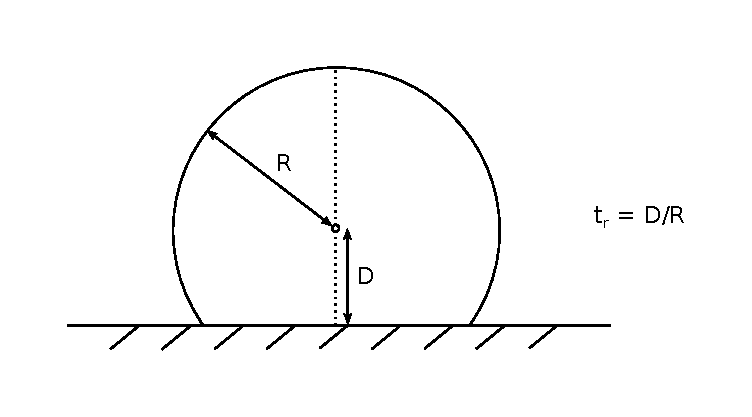
\includegraphics[width=0.5\textwidth]{truncationRatio.pdf}
   %\caption{
   %The geometrical meaning of the truncation ratio.
   %}
   %\label{fig:energyComparison}
%\end{figure}
%%
%\begin{table}[htbp]
   %\caption{oppbyggningen av ''.nk'' filene i Sopra-Databasen}
%\centering
%\begin{tabular}{ c c c c c }
%\hline
 %\multicolumn{2}{c}{unit}         &  startverdi  &  sluttverdi & antall datapunkter \\
%\hline
%1          & 2                    &                 &                  & \\
%energi[eV] & bølgelengde[$\mu$m]  &  x1[eV/$\mu$m]  &    x2[eV/$\mu$m] & N \\
%\hline
%\end{tabular}
%\label{tab:idealTCW}
%\end{table}
%%


